\documentclass[12pt,a4paper]{article}

% ==================== PAQUETES ====================
\usepackage{fontspec}
\usepackage[spanish]{babel}
\usepackage{geometry}
\usepackage{graphicx}
\usepackage{booktabs}
\usepackage{amsmath}
\usepackage{amssymb}
\usepackage{enumitem}
\usepackage{hyperref}
\usepackage{xcolor}
\usepackage{listings}
\usepackage{caption}
\usepackage{float}
\usepackage{longtable}
\usepackage{fancyhdr}
\usepackage{titlesec}

\graphicspath{{../imgs/}} 

\geometry{left=3cm, right=2.5cm, top=2.5cm, bottom=2.5cm, headheight=14.5pt}

\hypersetup{
    colorlinks=true,
    linkcolor=black,
    citecolor=blue,
    urlcolor=blue
}

\lstset{
    basicstyle=\ttfamily\footnotesize,
    breaklines=true,
    frame=single,
    backgroundcolor=\color{gray!10},
    numbers=left,
    numberstyle=\tiny,
    keywordstyle=\color{blue},
    commentstyle=\color{green!50!black},
    stringstyle=\color{red!70!black},
    showstringspaces=false
}

\renewcommand{\tablename}{Tabla}

\pagestyle{fancy}
\fancyhf{}
\rhead{Sistema de Riego Inteligente con TinyML}
\lhead{UNSAAC --- EPIIS}
\rfoot{\thepage}


\titleformat{\section}{\normalfont\Large\bfseries}{\thesection}{1em}{}
\titleformat{\subsection}{\normalfont\large\bfseries}{\thesubsection}{1em}{}


% ==================== DOCUMENTO ====================
\begin{document}

%--- PORTADA ---------------------------------------------------
\begin{titlepage}
  \centering
  \vspace{1.5cm}
  {\Huge\bfseries Sistema de Riego Inteligente \par}
  \vspace{0.5cm}
  {\large Basado en TinyML sobre ESP32 \par}
  \vspace{1.5cm}
  \rule{\linewidth}{0.5pt}
  \vspace{1cm}

  {\large\textbf{Asignatura:} Sistemas Embebidos\par}
  \vspace{0.3cm}
  {\large\textbf{Docente:} Mgt. Jose Mauro Pillco Quispe\par}
  \vspace{0.3cm}


  
  \textbf{Integrantes:}
  \begin{itemize}[leftmargin=4cm]
    \item Joseph Jesus Callañaupa Salcedo
    \item Denis Jair Cancinas Cardenas
  \end{itemize}\vspace{1.2cm}

  \rule{\linewidth}{0.5pt}
  \vspace{1cm}

  \textbf{Repositorio GitHub:}\\
  \url{}\\
  \vspace{0.5cm}
  \textbf{Conversación de desarrollo:}\\
  \url{https://claude.ai/share/84b34524-631f-4bdc-92d9-efbb7071c85a}\\
  \vspace{1cm}

  {\large Cusco, Perú --- 2026\par}
\end{titlepage}

\newpage

\tableofcontents
\newpage

% ==================== RESUMEN ====================
\section*{Resumen}
\addcontentsline{toc}{section}{Resumen}

El presente informe describe el diseño, implementación y validación experimental de un sistema de riego inteligente autónomo basado en Edge AI y TinyML, desplegado sobre un microcontrolador ESP32. El sistema integra un sensor capacitivo de humedad de suelo (HW-390) y un sensor digital de temperatura y humedad ambiental (AHT10), cuyas lecturas alimentan un modelo de clasificación de aprendizaje automático (red neuronal densa cuantizada a 8 bits) ejecutado localmente en el dispositivo mediante TensorFlow Lite Micro. El modelo clasifica el estado del sustrato en tres categorías --SECO, ÓPTIMO y SATURADO-- a partir de las cuales se deriva una recomendación de riego. Se recolectaron y etiquetaron manualmente más de 5{,}000 muestras reales bajo distintas condiciones de temperatura ambiental, identificándose y cuantificándose un efecto de confusión térmica sobre la lectura del sensor capacitivo, el cual fue mitigado incorporando la temperatura como variable de entrada adicional del modelo. El clasificador final alcanzó una exactitud del 99.42\% sobre el conjunto de prueba. Los resultados se transmiten mediante HTTP hacia un servidor Node.js alojado en AWS EC2, el cual expone un panel de control (dashboard) en tiempo real vía WebSocket. Debido a restricciones de disponibilidad de hardware, la validación experimental se limitó al módulo de sensado, inferencia y visualización (modo de observación o \textit{shadow mode}), quedando la integración del lazo de actuación (electroválvula/bomba) como trabajo futuro inmediato.\\

\vspace{0.3cm}
\noindent \textbf{Palabras clave:} TinyML, Edge Computing, Internet de las Cosas, Agricultura de Precisión, Riego Inteligente, TensorFlow Lite Micro, ESP32.

\newpage

% ==================== INTRODUCCION ====================
\section{Introducción}

La agricultura de precisión ha encontrado en el Internet de las Cosas (IoT) y en el aprendizaje automático embebido (TinyML) un conjunto de herramientas capaces de optimizar el uso de recursos hídricos sin requerir infraestructura costosa ni dependencia constante de conectividad a internet. En contextos de escasez hídrica y variabilidad climática, los sistemas de riego automatizados que basan sus decisiones en umbrales fijos resultan insuficientes, ya que no logran adaptarse a condiciones ambientales cambiantes ni a las particularidades del sustrato sobre el que se opera.\\

El paradigma de \textit{Edge AI} propone trasladar la inferencia del modelo de aprendizaje automático desde la nube hacia el propio dispositivo embebido, lo cual reduce la latencia de decisión, elimina la dependencia de conectividad permanente y disminuye el consumo energético asociado a la transmisión constante de datos crudos. TinyML es la disciplina que hace posible ejecutar estos modelos dentro de las restricciones de memoria y cómputo propias de un microcontrolador.\\

El presente trabajo documenta el desarrollo completo de un sistema de riego inteligente que aplica estos principios: captura de variables ambientales y de sustrato mediante sensores de bajo costo, entrenamiento de un modelo de clasificación supervisado, conversión y cuantización del modelo para su ejecución en un ESP32, y visualización remota de resultados mediante un panel web conectado a un servidor en la nube.

% ==================== PLANTEAMIENTO DEL PROBLEMA ====================
\section{Planteamiento del Problema}

\subsection{Situación problemática}
La escasez hídrica y la variabilidad climática representan desafíos crecientes para la agricultura, particularmente en pequeños productores y agricultura doméstica o de traspatio, donde el riego suele realizarse de forma manual o mediante temporizadores fijos que no consideran el estado real del sustrato ni las condiciones ambientales del momento. Esta práctica conduce recurrentemente a dos escenarios indeseables: el riego insuficiente, que provoca estrés hídrico en el cultivo, y el riego excesivo, que genera saturación del sustrato, pérdida de nutrientes por lixiviación y condiciones propicias para enfermedades radiculares.\\

Los sistemas de riego automatizados de bajo costo disponibles comercialmente suelen basar su decisión en un único sensor de humedad de suelo evaluado contra un umbral fijo predefinido. Sin embargo, la evidencia experimental recabada en el presente trabajo (Sección \ref{sec:resultados}) demuestra que los sensores capacitivos de humedad de suelo --tecnología preferida sobre los sensores resistivos por su mayor durabilidad-- presentan una sensibilidad térmica considerable: su lectura analógica varía de forma significativa con la temperatura ambiental incluso cuando el contenido real de humedad del sustrato permanece constante. Este fenómeno, escasamente documentado en las hojas de datos comerciales de estos módulos y no cuantificado explícitamente en la literatura revisada (Sección \ref{sec:estado_arte}), introduce un sesgo sistemático que invalida la premisa de estabilidad requerida por cualquier esquema de decisión basado en un umbral único.\\

Adicionalmente, el paradigma predominante en sistemas IoT agrícolas de bajo costo depende de conectividad permanente a internet para el procesamiento de decisiones en la nube, lo cual introduce puntos de falla ante interrupciones de red y añade latencia y consumo energético innecesarios para una decisión que, en principio, podría resolverse localmente en el propio dispositivo de sensado.

\subsection{Formulación del problema}

\subsubsection{Problema general}
¿Cómo diseñar e implementar un sistema de riego autónomo, basado en un modelo de clasificación TinyML embebido en un microcontrolador ESP32, que tome decisiones de riego robustas frente a la variabilidad térmica ambiental, sin requerir conectividad permanente a internet para su funcionamiento?

\subsubsection{Problemas específicos}
\begin{itemize}
    \item[$PE_1$:] ¿En qué medida la temperatura ambiental afecta la lectura del sensor capacitivo de humedad de suelo, y hasta qué punto un esquema de decisión basado en un único umbral fijo resulta insuficiente para compensar dicho efecto?
    \item[$PE_2$:] ¿En qué medida la incorporación de variables ambientales adicionales (temperatura y humedad relativa) mejora la exactitud de un modelo de clasificación del estado hídrico del sustrato, respecto de un modelo que emplea únicamente la lectura del sensor de suelo?
    \item[$PE_3$:] ¿Es posible desplegar un modelo de clasificación de aprendizaje automático, cuantizado a 8 bits, dentro de las restricciones de memoria y procesamiento de un microcontrolador ESP32, preservando su capacidad de clasificación correcta en condiciones de hardware real?
    \item[$PE_4$:] ¿Cómo integrar el dispositivo de borde con un canal de comunicación y un sistema de visualización remota en tiempo real, sin que la disponibilidad de dicho canal sea un requisito para la toma de decisiones del sistema?
\end{itemize}

\subsection{Justificación}
El presente trabajo se justifica desde tres perspectivas. Desde una perspectiva \textbf{tecnológica}, aporta evidencia cuantitativa de un fenómeno --la sensibilidad térmica del sensor capacitivo de humedad de suelo-- que, pese a su relevancia práctica para el diseño de sistemas de riego de precisión, no se encuentra explícitamente cuantificado en los antecedentes revisados. Desde una perspectiva \textbf{ambiental y económica}, un sistema de riego que responde al estado real del sustrato en lugar de horarios fijos contribuye a la optimización del uso del recurso hídrico, consistente con los hallazgos de eficiencia reportados en la literatura de riego de precisión basado en TinyML. Desde una perspectiva \textbf{académica}, el trabajo documenta un caso de aplicación completo del paradigma Edge AI --desde la recolección de datos hasta el despliegue en hardware real-- que puede servir como referencia metodológica para proyectos similares dentro de la Escuela Profesional de Ingeniería Informática y de Sistemas.

\subsection{Delimitación}
El presente estudio se circunscribe al diseño, entrenamiento y validación del módulo de sensado, inferencia y visualización del sistema, empleando un macetero individual como caso de estudio experimental. La integración física del módulo de actuación (electroválvula o bomba de agua) y la validación en condiciones de campo abierto con múltiples cultivos quedan fuera del alcance del presente trabajo, y se documentan como limitaciones (Sección \ref{sec:limitaciones}) y trabajo futuro.

% ==================== OBJETIVOS ====================
\section{Objetivos}

\subsection{Objetivo general}
Implementar y validar experimentalmente un sistema de riego inteligente basado en Edge AI, que utilice un modelo de clasificación TinyML ejecutado localmente en un microcontrolador ESP32 para determinar el estado hídrico del sustrato a partir de variables de suelo y ambientales, de forma robusta ante la variabilidad térmica ambiental y sin depender de conectividad permanente a internet.

\subsection{Objetivos específicos}
\begin{itemize}
    \item[$OE_1$:] Cuantificar el efecto de la temperatura ambiental sobre la lectura del sensor capacitivo de humedad de suelo HW-390, y evaluar la insuficiencia de un esquema de decisión basado en un único umbral fijo para compensar dicho efecto.
    \item[$OE_2$:] Determinar la mejora en exactitud de clasificación obtenida al incorporar temperatura y humedad ambiental como variables adicionales de un modelo de clasificación del estado hídrico del sustrato, respecto de un modelo univariable.
    \item[$OE_3$:] Desplegar un modelo de red neuronal de clasificación cuantizado mediante TensorFlow Lite Micro sobre un microcontrolador ESP32, evaluando su consumo de recursos de memoria y verificando la consistencia de sus clasificaciones respecto al modelo original en punto flotante, en condiciones de hardware real.
    \item[$OE_4$:] Implementar un canal de comunicación HTTP y un panel de visualización remota en tiempo real que reciba las predicciones del dispositivo de borde, sin comprometer la autonomía de decisión del sistema ante la ausencia de dicho canal.
\end{itemize}

\noindent \textit{Nota metodológica}: cada objetivo específico ($OE_i$) atiende directamente al problema específico correspondiente ($PE_i$) formulado en la Sección 2.2.2, y su cumplimiento se valida mediante la hipótesis específica homóloga ($H_i$) presentada a continuación.

% ==================== HIPOTESIS ====================
\section{Hipótesis}

\subsection{Hipótesis general}
Un sistema de riego basado en un modelo de clasificación TinyML embebido en un microcontrolador ESP32, que incorpora la temperatura ambiental y la humedad relativa como variables de entrada además de la lectura del sensor de humedad de suelo, permite tomar decisiones de riego robustas frente a la variabilidad térmica ambiental y operar de forma autónoma sin depender de conectividad permanente a internet.

\subsection{Hipótesis específicas}
\begin{itemize}
    \item[$H_1$:] La lectura cruda del sensor capacitivo de humedad de suelo (variable dependiente) presenta una correlación estadísticamente significativa con la temperatura ambiental (variable independiente) para un mismo estado real de humedad del sustrato. Como consecuencia, un esquema de decisión basado en un único umbral fijo resulta insuficiente para clasificar correctamente dicho estado.
    \item[$H_2$:] Un modelo de clasificación entrenado incorporando \textit{soil\_raw}, temperatura y humedad ambiental como variables independientes alcanza una exactitud de clasificación significativamente superior --en al menos 10 puntos porcentuales-- respecto de un modelo entrenado únicamente con \textit{soil\_raw}.
    \item[$H_3$:] Un modelo de red neuronal densa cuantizado a 8 bits mediante TensorFlow Lite Micro puede ejecutarse dentro de las restricciones de memoria RAM y flash de un microcontrolador ESP32, produciendo clasificaciones correctas y consistentes con las obtenidas por el modelo original en condiciones de hardware real.
    \item[$H_4$:] Un canal de comunicación HTTP y un panel de visualización remota en tiempo real pueden integrarse al dispositivo de borde sin comprometer su autonomía de decisión ni incrementar la latencia de inferencia local.
\end{itemize}

% ==================== MARCO TEORICO ====================
\section{Marco Teórico}

\subsection{Internet de las Cosas (IoT) en agricultura de precisión}
El Internet de las Cosas describe la interconexión de dispositivos físicos equipados con sensores y capacidad de comunicación, que permiten la captura, transmisión y procesamiento de datos del entorno físico. Aplicado a la agricultura, el IoT posibilita el monitoreo continuo de variables como humedad de suelo, temperatura, luminosidad y precipitación, sustituyendo la inspección manual por sistemas de sensado automatizado.

\subsection{Edge Computing y Edge AI}
El \textit{Edge Computing} traslada el procesamiento de datos desde servidores centralizados (la nube) hacia el borde de la red, es decir, hacia el propio dispositivo que genera los datos. Cuando este procesamiento incluye la ejecución de modelos de aprendizaje automático, se denomina \textit{Edge AI}. Sus principales ventajas frente al procesamiento en la nube son: reducción de la latencia de decisión, funcionamiento autónomo ante interrupciones de conectividad, menor consumo energético por transmisión de datos, y mayor privacidad al no requerir el envío de datos crudos hacia terceros.

\subsection{TinyML}
TinyML es la subdisciplina del aprendizaje automático orientada a la ejecución de modelos de inferencia en dispositivos con severas restricciones de memoria (típicamente cientos de kilobytes de RAM) y de cómputo, como los microcontroladores. Para lograr esta ejecución, los modelos entrenados en plataformas convencionales (por ejemplo, TensorFlow/Keras) deben someterse a un proceso de conversión y optimización:

\begin{enumerate}
    \item \textbf{Conversión a TensorFlow Lite}: el modelo se serializa en un formato compacto (\texttt{.tflite}) mediante \textit{FlatBuffers}.
    \item \textbf{Cuantización}: los pesos y activaciones del modelo, originalmente representados en punto flotante de 32 bits, se convierten a enteros de 8 bits (\textit{int8}), reduciendo el tamaño del modelo hasta en un factor de 4 con una pérdida de exactitud generalmente marginal.
    \item \textbf{Despliegue mediante TensorFlow Lite Micro}: un intérprete en lenguaje C++ optimizado para microcontroladores ejecuta el modelo cuantizado directamente sobre el hardware embebido.
\end{enumerate}

\subsection{Sensores capacitivos de humedad de suelo}
A diferencia de los sensores resistivos, que miden la resistencia eléctrica entre dos electrodos expuestos y son propensos a la corrosión por electrólisis, los sensores capacitivos miden la permitividad dieléctrica del sustrato, la cual varía en función de su contenido de agua. Esta tecnología ofrece mayor durabilidad, pero conserva una sensibilidad térmica no trivial: la permitividad dieléctrica medida por el sensor se ve afectada por la temperatura del sustrato y del propio circuito de medición, fenómeno que se cuantifica experimentalmente en la Sección \ref{sec:resultados}.

\subsection{Redes neuronales densas y cuantización}
El modelo de clasificación empleado en este trabajo corresponde a una red neuronal densa (\textit{feed-forward}) de baja complejidad, compuesta por una capa oculta con activación ReLU y una capa de salida con activación \textit{softmax} para la clasificación multiclase. La cuantización post-entrenamiento (\textit{post-training quantization}) transforma los pesos flotantes a enteros de 8 bits mediante un conjunto representativo de datos de calibración, preservando la escala y el punto cero (\textit{zero-point}) necesarios para reconstruir aproximadamente los valores originales durante la inferencia.

% ==================== ESTADO DEL ARTE ====================
\section{Estado del Arte}
\label{sec:estado_arte}

La revisión de trabajos previos permite identificar tendencias consistentes en la aplicación de TinyML y Edge AI a sistemas de riego y monitoreo agrícola, así como buenas prácticas de diseño arquitectónico y limitaciones recurrentes que este trabajo busca abordar.\\

Taueatsoala et al. \cite{taueatsoala2026} proponen un marco de IoT de cuatro capas para riego de precisión sostenible, integrando un ESP32 como dispositivo de borde y una Raspberry Pi como servidor de borde, sin dependencia de conectividad a la nube. Los autores evaluaron algoritmos de \textit{Gradient Boosting} y \textit{Random Forest} para la predicción de necesidad de riego, encontrando que el primero superó al segundo (R² de 0.9973 frente a 0.9916), y que el modelo desplegado en TinyML alcanzó un error porcentual absoluto medio (MAPE) inferior al 1\%, validando la viabilidad de la inferencia local para reducir el consumo hídrico.\\

Surbakti et al. \cite{surbakti2025} implementaron un modelo de regresión logística embebido en ESP32 para la clasificación de condiciones de humedad de suelo en cultivos de arroz, entrenado sobre datos de microclima local en Indonesia (3{,}021 registros). El modelo alcanzó una exactitud de 93.4\% y un F1-score ponderado de 0.927 sobre el conjunto de prueba, demostrando que modelos relativamente simples pueden ofrecer resultados robustos en este dominio cuando se dispone de un volumen de datos adecuado.\\

Thirumalaiah et al. \cite{thirumalaiah2025} presentan una arquitectura de referencia terminal-borde-nube para Edge AI en agricultura inteligente, combinando sensores ambientales y de visión con conectividad LoRaWAN, orientada tanto al riego inteligente como a la detección de enfermedades en plantas. Los autores plantean esta arquitectura como una propuesta conceptual, dejando la validación experimental de ahorro hídrico y desempeño de inferencia como trabajo futuro, patrón metodológico que este informe replica parcialmente al documentar una arquitectura completa cuya validación experimental se circunscribe al módulo de sensado e inferencia.\\

Kadhum et al. \cite{kadhum2025} desarrollaron un marco de TinyML optimizado mediante mecanismos de atención para el procesamiento de datos de sensores agrícolas en microcontroladores ESP32 y STM32, empleando entrenamiento consciente de cuantización (\textit{Quantization-Aware Training}) y búsqueda de arquitectura neuronal (\textit{Neural Architecture Search}). El sistema propuesto alcanzó una exactitud de clasificación de 96.8\%, con tiempos de inferencia inferiores a 15 ms y un tamaño de modelo por debajo de 100 KB en memoria flash, evidenciando la viabilidad de modelos considerablemente más sofisticados que el aquí presentado para escenarios de mayor exigencia.\\

Samanta y Saha \cite{samanta2026} realizan una revisión orientada al despliegue de sistemas de Edge AI y TinyML de bajo costo para agricultura de precisión en entornos con recursos limitados, identificando que los microcontroladores ESP32, STM32 y ATMega dominan las implementaciones revisadas, y que la cuantización constituye la técnica de optimización más adoptada, presente en aproximadamente el 50\% de los estudios analizados. Los autores señalan además una notable inconsistencia en el reporte de métricas de utilización de recursos entre los distintos trabajos, dificultando la comparación y reproducibilidad de resultados.\\

Finalmente, Rahman \cite{rahman2025} describe un sistema de riego inteligente basado en microcontrolador con lógica de decisión impulsada por inteligencia artificial, empleando TensorFlow Lite for Microcontrollers sobre un ESP32 con registro opcional en la nube mediante Firebase. El sistema reportó una reducción del consumo de agua de hasta 38\% y un incremento del rendimiento de cultivo cercano al 12\% en pruebas de campo con lechuga y tomate, si bien la validación se limitó a estas dos especies vegetales.\\

En conjunto, la literatura revisada confirma una convergencia hacia el uso de microcontroladores de bajo costo (predominantemente ESP32), la adopción extendida de la cuantización como técnica de optimización, y una inclinación hacia la inferencia local para preservar la autonomía del sistema ante la ausencia de conectividad. Sin embargo, ninguno de los trabajos revisados cuantifica explícitamente el efecto de la temperatura ambiental sobre la lectura del sensor de humedad de suelo, aspecto que constituye un aporte específico del presente trabajo.

% ==================== METODOLOGIA ====================
\section{Metodología}

\subsection{Arquitectura del sistema}
El sistema se estructura en cuatro componentes principales: (1) el dispositivo de borde (ESP32 con sensores e inferencia local), (2) el canal de comunicación HTTP, (3) el servidor de aplicación (Node.js sobre AWS EC2), y (4) el panel de visualización web en tiempo real mediante WebSocket. La Figura \ref{fig:arquitectura} presenta el diagrama completo de la arquitectura propuesta, incluyendo el módulo de actuación (electroválvula y relé), cuya integración física queda documentada como trabajo futuro en la Sección \ref{sec:limitaciones}.

\begin{figure}[H]
    \centering
    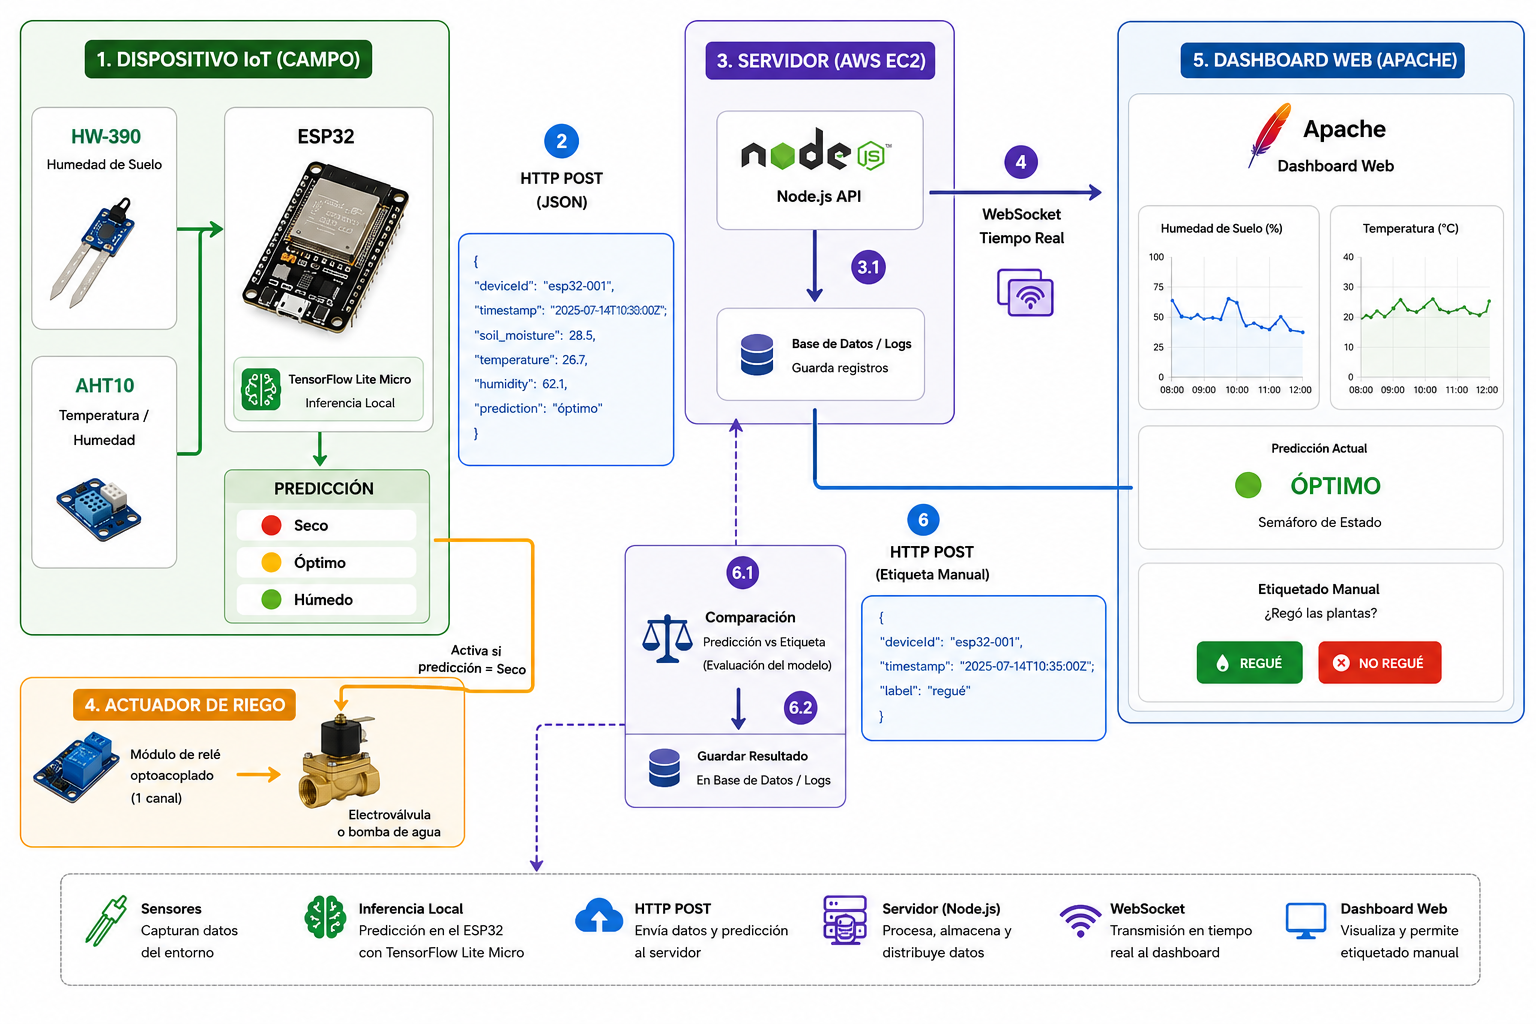
\includegraphics[width=0.9\textwidth]{arquitectura.png}
    \caption{Arquitectura general del sistema de riego inteligente.}
    \label{fig:arquitectura}
\end{figure}

\subsection{Hardware}
\begin{itemize}
    \item \textbf{Microcontrolador}: ESP32 DEVKIT V1 (WROOM-32), framework Arduino.
    \item \textbf{Sensor de humedad de suelo}: HW-390, sensor capacitivo de 3 pines (AOUT, VCC, GND), salida analógica conectada al pin ADC \texttt{GPIO34}.
    \item \textbf{Sensor de temperatura y humedad ambiental}: AHT10, comunicación I2C (dirección \texttt{0x38}), conectado a los pines \texttt{GPIO21} (SDA) y \texttt{GPIO22} (SCL).
\end{itemize}

La Figura \ref{fig:circuito} muestra el diagrama de conexión del circuito real implementado, y la Figura \ref{fig:circuito_wokwi} el circuito equivalente empleado durante la fase de simulación en el entorno Wokwi, previa a la disponibilidad del hardware físico.

\begin{figure}[H]
    \centering
    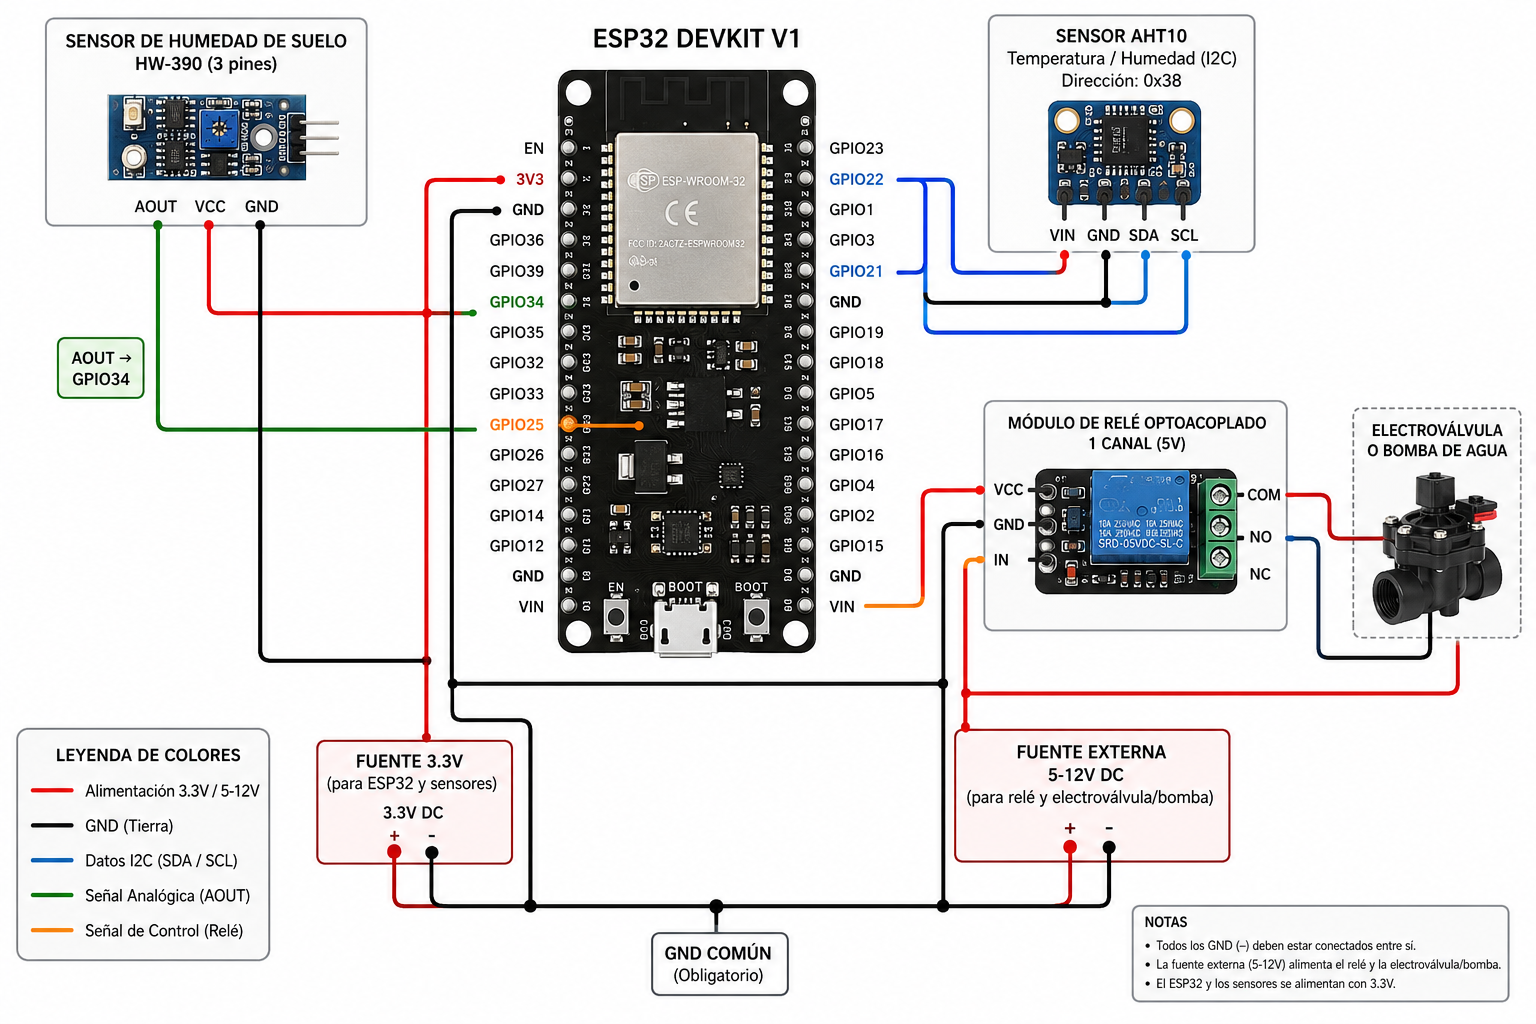
\includegraphics[width=0.85\textwidth]{circuito.png}
    \caption{Diagrama de conexión del circuito físico (ESP32, HW-390 y AHT10).}
    \label{fig:circuito}
\end{figure}

\begin{figure}[H]
    \centering
    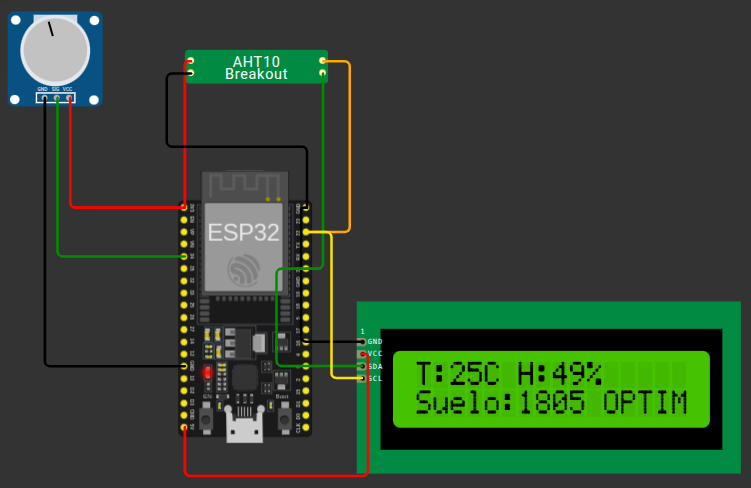
\includegraphics[width=0.7\textwidth]{circuito_wokwi.png}
    \caption{Circuito de simulación implementado en el entorno Wokwi.}
    \label{fig:circuito_wokwi}
\end{figure}

\subsection{Software y flujo de procesamiento}
El firmware del ESP32, desarrollado en PlatformIO sobre framework Arduino, ejecuta el ciclo descrito en la Figura \ref{fig:flujo}: lectura de sensores, normalización de variables, cuantización a enteros de 8 bits, inferencia mediante el intérprete de TensorFlow Lite Micro (biblioteca \texttt{Chirale\_TensorFlowLite}), y transmisión del resultado hacia el servidor remoto mediante solicitudes HTTP POST.

\begin{figure}[H]
    \centering
    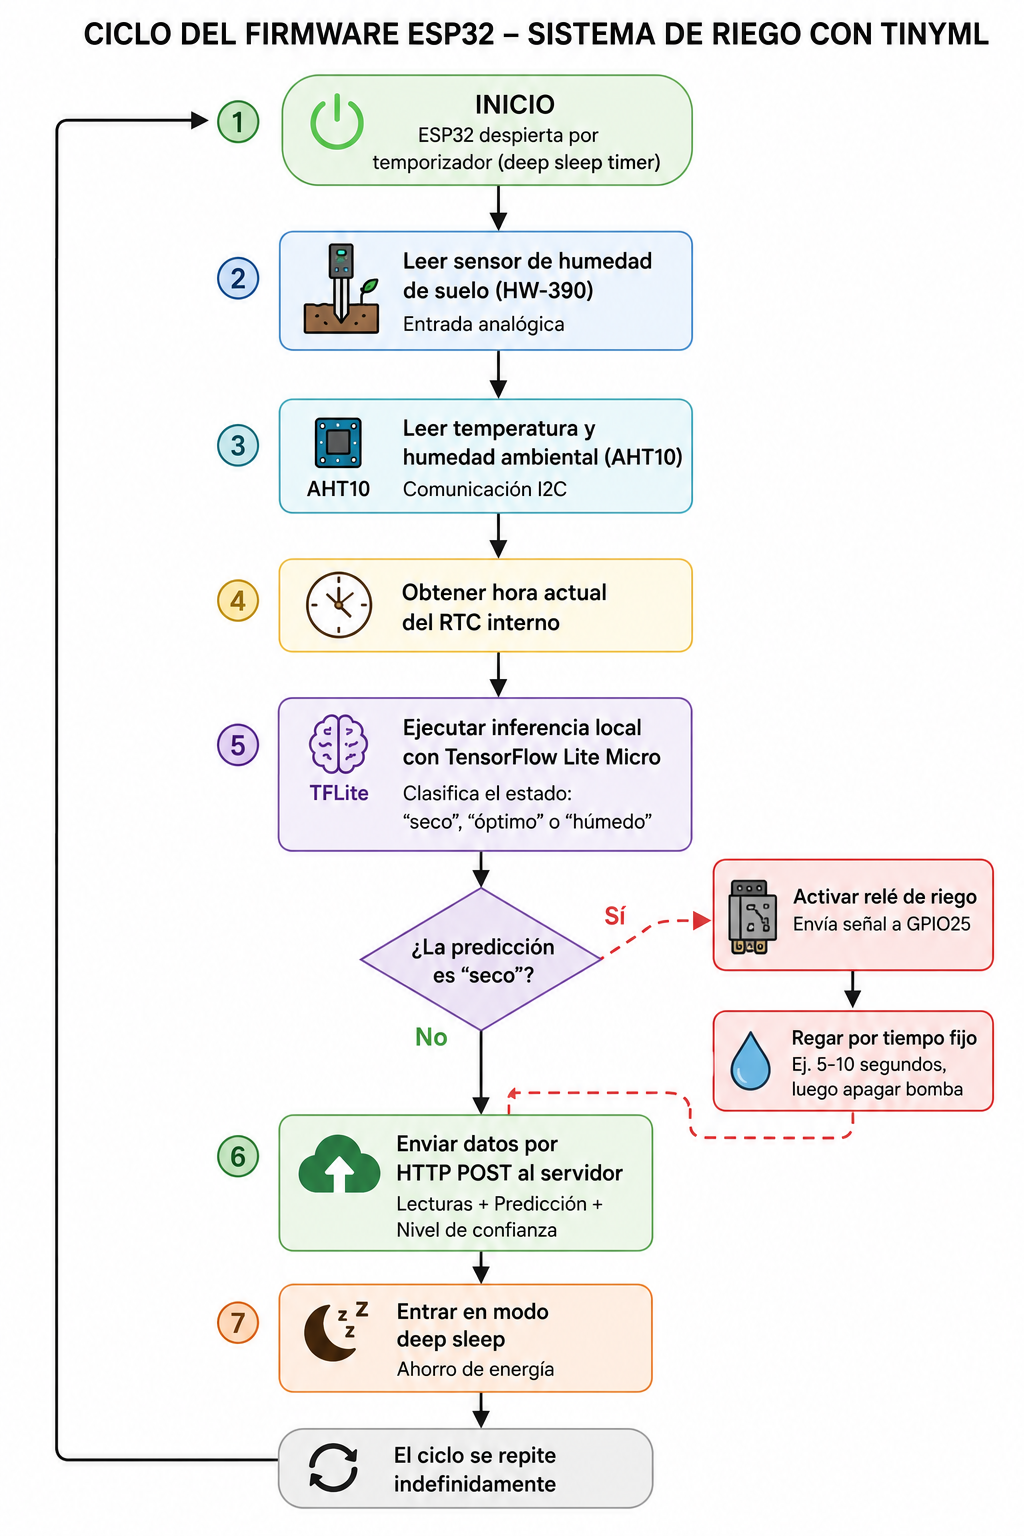
\includegraphics[width=0.55\textwidth]{flujo.png}
    \caption{Diagrama de flujo del firmware embebido en el ESP32.}
    \label{fig:flujo}
\end{figure}

La conectividad WiFi se gestiona mediante la biblioteca \texttt{WiFiManager}, que implementa un portal cautivo de aprovisionamiento: ante la ausencia de credenciales guardadas, el dispositivo crea su propio punto de acceso, permitiendo al usuario configurar la red WiFi de destino desde cualquier dispositivo móvil sin necesidad de recompilar el firmware.

\subsection{Recolección y etiquetado del conjunto de datos}
Se recolectaron muestras mediante sesiones controladas en las que se regó manualmente un macetero de prueba y registró, junto a cada lectura de los sensores, una etiqueta de estado observado (\textit{seco}, \textit{húmedo}, \textit{mojado}), determinada por criterio agronómico directo (tacto y observación visual del sustrato) y no por umbrales del propio sensor. Las sesiones se distribuyeron en distintos momentos del día (mañana, tarde, noche) para capturar la variabilidad térmica ambiental natural. El conjunto de datos final consolidado comprende 5{,}178 muestras.\\

Las cuatro categorías observadas se remapearon a un esquema de tres clases orientado a la decisión de riego:
\begin{itemize}
    \item \textbf{SECO}: requiere riego inmediato.
    \item \textbf{ÓPTIMO}: rango adecuado, sin necesidad de acción.
    \item \textbf{SATURADO}: exceso de agua, condición de alerta.
\end{itemize}

La Tabla \ref{tab:muestra_datos} presenta una muestra representativa del conjunto de datos recolectado.

\begin{table}[H]
\centering
\caption{Muestra representativa del conjunto de datos recolectado.}
\label{tab:muestra_datos}
\small
\begin{tabular}{@{}rrrlll@{}}
\toprule
\textbf{soil\_raw} & \textbf{temp (°C)} & \textbf{hum (\%)} & \textbf{estado} & \textbf{momento} & \textbf{label} \\
\midrule
1178 & 22.48 & 28.01 & humedo       & día    & OPTIMO   \\
1275 & 13.72 & 40.68 & humedo       & noche  & OPTIMO   \\
1392 & 18.62 & 24.06 & humedo       & tarde  & OPTIMO   \\
1892 & 28.75 & 21.58 & humedo        & día    & OPTIMO   \\
1525 & 18.36 & 23.35 & humedo        & tarde  & OPTIMO   \\
1062 & 21.99 & 28.06 & mojado        & día    & SATURADO \\
1006 & 13.69 & 41.72 & mojado        & noche  & SATURADO \\
2785 & 23.93 & 27.43 & seco          & día    & SECO     \\
2000 & 14.77 & 36.96 & seco          & noche  & SECO     \\
2064 & 17.98 & 24.29 & seco          & tarde  & SECO     \\
1948 & 18.76 & 21.80 & seco          & tarde  & OPTIMO   \\
2511 & 31.36 & 26.68 & humedo        & día    & SECO     \\
\bottomrule
\end{tabular}
\end{table}

\noindent \textit{Nota}: las dos últimas filas de la tabla corresponden a casos límite en los que el efecto de la temperatura ambiental provoca una lectura cruda del sensor inconsistente con la etiqueta de umbral fijo, evidencia empírica que motiva el uso de un modelo multivariable (ver Sección \ref{sec:resultados}).

\subsection{Justificación del uso de un modelo de aprendizaje automático frente a un esquema de umbrales fijos}

Previo al diseño del modelo de clasificación, se evaluó la viabilidad de un esquema de decisión más simple basado en umbrales fijos sobre la lectura cruda del sensor de humedad de suelo (por ejemplo, \textit{si soil\_raw $\geq$ 1950, entonces SECO}), enfoque ampliamente utilizado en sistemas de riego automatizados de bajo costo. Sin embargo, este esquema presenta una limitación estructural: un umbral fijo solo puede trazar una frontera de decisión unidimensional, incapaz de adaptarse a variaciones en las demás condiciones ambientales bajo las cuales se realiza la medición.\\

Como se demuestra empíricamente en la Sección \ref{sec:resultados}, la lectura del sensor capacitivo HW-390 no depende únicamente del contenido real de humedad del sustrato, sino que se ve afectada de forma sistemática por la temperatura ambiental. En consecuencia, un mismo valor de \textit{soil\_raw} puede corresponder a estados de humedad real distintos según la temperatura al momento de la medición, lo cual invalida la premisa fundamental de cualquier esquema de umbral único: que la variable de entrada guarda una relación monótona y estable con la clase que se desea predecir.\\

Frente a esta limitación, un modelo de aprendizaje automático supervisado ofrece dos ventajas concretas para este problema:

\begin{itemize}
    \item \textbf{Capacidad de aprender fronteras de decisión multivariables}: al incorporar \textit{soil\_raw}, temperatura y humedad ambiental como variables de entrada simultáneas, el modelo puede aprender una frontera de decisión no lineal que compensa el efecto de la temperatura sobre la lectura del sensor, en lugar de asumir una relación fija e independiente del contexto ambiental.
    \item \textbf{Generalización a partir de datos observados, no de supuestos de diseño}: mientras que un umbral fijo requiere que el desarrollador determine manualmente el punto de corte correcto --frecuentemente mediante prueba y error--, el modelo entrenado infiere dicha frontera directamente a partir de las relaciones presentes en los datos etiquetados, lo cual resulta más robusto ante las particularidades del sustrato y del sensor específico empleado.
\end{itemize}

Esta decisión de diseño se valida cuantitativamente en la Sección \ref{sec:resultados}, donde se comparan directamente el desempeño de un modelo univariable (equivalente en espíritu a un esquema de umbral) frente al modelo multivariable propuesto, sobre un mismo conjunto de datos de prueba.

\subsection{Entrenamiento del modelo}
El modelo se entrenó en el entorno Google Colab utilizando la biblioteca Keras (TensorFlow), con la siguiente arquitectura:

\begin{lstlisting}[language=Python, caption={Arquitectura del modelo de clasificación.}]
modelo = keras.Sequential([
    keras.layers.Input(shape=(3,)),
    keras.layers.Dense(8, activation='relu'),
    keras.layers.Dense(3, activation='softmax')
])
\end{lstlisting}

Las variables de entrada (\textit{soil\_raw}, \textit{temperatura}, \textit{humedad ambiental}) se estandarizaron mediante \texttt{StandardScaler} previo al entrenamiento. El modelo entrenado se convirtió a formato TensorFlow Lite y se cuantizó a enteros de 8 bits mediante un conjunto de calibración representativo, obteniendo un modelo final de 2{,}280 bytes, exportado como arreglo en lenguaje C para su inclusión directa en el firmware del ESP32.

% ==================== RESULTADOS ====================
\section{Resultados}
\label{sec:resultados}

\subsection{Efecto de la temperatura sobre el sensor de humedad de suelo}
El análisis exploratorio del conjunto de datos recolectado evidenció una correlación considerable entre la temperatura ambiental y la lectura cruda del sensor HW-390 para un mismo estado real de humedad del sustrato. En la clase SECO, por ejemplo, las lecturas oscilaron entre 1{,}935 y 3{,}056 unidades del conversor analógico-digital según la temperatura ambiental registrada (13.6\,°C a 31.6\,°C), un rango de variación (1{,}121 unidades) comparable a la separación completa entre las clases SECO y SATURADO. Esta evidencia confirma la hipótesis $H_1$ y justifica empíricamente la incorporación de la temperatura como variable de entrada adicional del modelo.

\subsection{Comparación: modelo univariable frente a modelo multivariable}
Se entrenó un modelo de referencia (regresión logística) utilizando únicamente la variable \textit{soil\_raw}, y se comparó contra un modelo equivalente que incorpora \textit{soil\_raw}, \textit{temperatura} y \textit{humedad ambiental}. Sobre un conjunto de validación externo de 180 muestras no utilizado durante el entrenamiento, el modelo univariable alcanzó una exactitud de 79\%, mientras que el modelo multivariable alcanzó 92\%, una mejora de 13 puntos porcentuales que confirma la hipótesis $H_2$.

\subsection{Desempeño del modelo final (red neuronal densa cuantizada)}
El modelo de red neuronal densa, entrenado sobre el conjunto de datos consolidado de 5{,}178 muestras y evaluado sobre una partición de prueba de 1{,}036 muestras (20\%), alcanzó una exactitud global de 99.42\%. La Tabla \ref{tab:metricas} resume las métricas de clasificación por clase, y la Figura \ref{fig:matriz_confusion} presenta la matriz de confusión correspondiente.

\begin{table}[H]
\centering
\caption{Métricas de clasificación del modelo final por clase.}
\label{tab:metricas}
\begin{tabular}{@{}lrrrr@{}}
\toprule
\textbf{Clase} & \textbf{Precisión} & \textbf{Recall} & \textbf{F1-score} & \textbf{Soporte} \\
\midrule
OPTIMO   & 1.00 & 0.98 & 0.99 & 351 \\
SATURADO & 0.98 & 1.00 & 0.99 & 343 \\
SECO     & 1.00 & 1.00 & 1.00 & 342 \\
\midrule
\textbf{Exactitud global} & \multicolumn{3}{r}{} & \textbf{99.42\% (1036)} \\
\bottomrule
\end{tabular}
\end{table}

\begin{figure}[H]
    \centering
    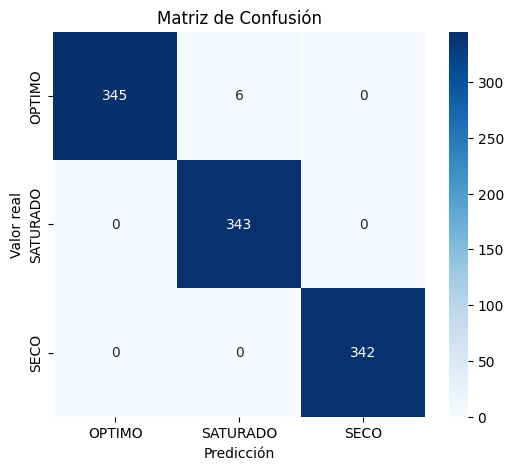
\includegraphics[width=0.6\textwidth]{matriz_confusion.png}
    \caption{Matriz de confusión del modelo de clasificación final sobre el conjunto de prueba.}
    \label{fig:matriz_confusion}
\end{figure}

Los seis errores de clasificación observados corresponden exclusivamente a la frontera entre las clases ÓPTIMO y SATURADO, consistente con el patrón de menor separabilidad identificado durante el análisis exploratorio para dicha región del espacio de variables.

\subsection{Validación en hardware real}
Tras la conversión y cuantización, el modelo (2{,}280 bytes) fue integrado en el firmware del ESP32 mediante la biblioteca \texttt{Chirale\_TensorFlowLite}, ejecutándose con un consumo de memoria de trabajo (\textit{tensor arena}) de 804 bytes, muy por debajo de la capacidad de RAM disponible en el microcontrolador (520 KB). Las pruebas de inferencia en tiempo real sobre hardware físico reprodujeron correctamente las predicciones esperadas conforme a los valores de calibración del sensor previamente establecidos (por ejemplo, lecturas de \textit{soil\_raw} superiores a 2{,}800 unidades fueron correctamente clasificadas como SECO).

\subsection{Panel de visualización remota}
El servidor Node.js desplegado en una instancia AWS EC2 recibe cada lectura mediante una solicitud HTTP POST, la almacena en un registro histórico local, y la transmite en tiempo real a un panel web mediante WebSocket. La Figura \ref{fig:dashboard} presenta la interfaz final del panel, que muestra el historial de variables mediante gráficos de series temporales, la predicción vigente representada mediante un indicador de color y un mensaje de acción recomendada (necesidad de riego, estado óptimo o exceso de agua), y una tabla con el historial reciente de lecturas.

\begin{figure}[H]
    \centering
    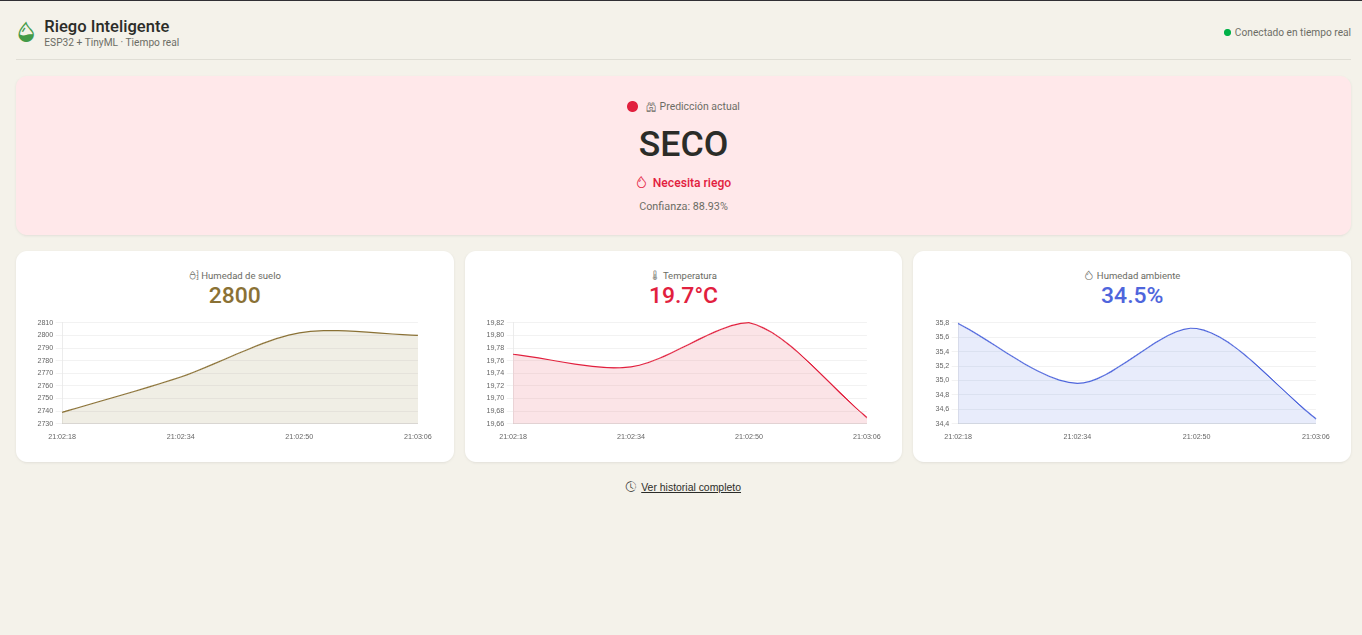
\includegraphics[width=0.9\textwidth]{dashboard.png}
    \caption{Panel de visualización web en tiempo real del sistema de riego inteligente.}
    \label{fig:dashboard}
\end{figure}

% ==================== DISCUSION ====================
\section{Discusión}

Los resultados obtenidos confirman las tres hipótesis planteadas en este trabajo. La correlación identificada entre la temperatura ambiental y la lectura del sensor capacitivo de humedad de suelo constituye un hallazgo relevante que, si bien es coherente con el comportamiento eléctrico esperado de este tipo de sensores, no se encuentra explícitamente cuantificado en los trabajos revisados en la Sección de Estado del Arte. La magnitud del efecto observado --una variación de más de 1{,}000 unidades del conversor analógico-digital atribuible únicamente a la temperatura, dentro de una misma clase de humedad real-- resulta suficientemente grande como para invalidar cualquier esquema de decisión basado en un único umbral fijo sobre la lectura cruda del sensor, particularmente en instalaciones expuestas a variaciones térmicas diarias o estacionales significativas, como es el caso de la región andina donde se realizó la presente investigación.\\

La mejora de 13 puntos porcentuales en exactitud al incorporar variables ambientales adicionales, y el desempeño final de 99.42\% del modelo de red neuronal densa, son consistentes con los resultados reportados por Surbakti et al. \cite{surbakti2025} (93.4\%) y superan a los de Taueatsoala et al. \cite{taueatsoala2026} en términos de simplicidad del modelo requerido, si bien ambos trabajos emplean esquemas de evaluación y conjuntos de datos distintos, lo que limita la comparabilidad directa, en línea con la observación de Samanta y Saha \cite{samanta2026} respecto a la inconsistencia en el reporte de métricas dentro de esta área de investigación.

% ==================== LIMITACIONES ====================
\section{Limitaciones}
\label{sec:limitaciones}

\begin{itemize}
    \item Si bien la arquitectura propuesta contempla el control activo del riego mediante electroválvula o bomba de agua y un módulo de relé (Figura \ref{fig:arquitectura}), la validación experimental del presente trabajo se limitó al módulo de sensado, inferencia y visualización (modo de observación), debido a restricciones de disponibilidad de hardware actuador al momento de la implementación. La integración del lazo de control completo queda como trabajo futuro inmediato.
    \item El conjunto de datos fue recolectado a partir de un único macetero y un único tipo de sustrato, lo cual limita la generalización directa del modelo entrenado a otros tipos de suelo o especies vegetales sin un proceso de recalibración o reentrenamiento adicional.
    \item La validación de hardware se realizó en un entorno doméstico controlado (interior de una vivienda), no en condiciones de campo abierto con exposición a precipitación, radiación solar directa o viento, variables no contempladas en el conjunto de sensores actual.
\end{itemize}

% ==================== CONCLUSIONES ====================
\section{Conclusiones}

\begin{enumerate}
    \item Se diseñó, implementó y validó experimentalmente un sistema de riego inteligente basado en Edge AI, capaz de clasificar el estado hídrico del sustrato en tres categorías mediante un modelo TinyML ejecutado localmente en un microcontrolador ESP32, sin dependencia de conectividad a internet para la toma de decisiones.
    \item Se cuantificó empíricamente el efecto de confusión térmica sobre el sensor capacitivo de humedad de suelo HW-390, demostrando que su lectura cruda no es un indicador confiable por sí solo del estado real de humedad del sustrato ante variaciones de temperatura ambiental.
    \item La incorporación de temperatura y humedad ambiental como variables adicionales del modelo de clasificación mejoró la exactitud en 13 puntos porcentuales respecto a un esquema de umbral único, y el modelo final de red neuronal densa cuantizada alcanzó una exactitud de 99.42\% sobre el conjunto de prueba.
    \item El modelo cuantizado (2{,}280 bytes) se ejecuta dentro de las restricciones de memoria del ESP32 con un margen amplio de recursos disponibles, confirmando la viabilidad de la cuantización post-entrenamiento para este tipo de aplicación.
    \item Se implementó un canal de comunicación y visualización remota funcional, mediante un servidor Node.js en AWS EC2 y un panel web en tiempo real, validando el flujo completo de datos desde el sensor hasta la interfaz de usuario final.
\end{enumerate}

% ==================== TRABAJO FUTURO ====================
\section{Trabajo Futuro}

\begin{itemize}
    \item Integración física del módulo de actuación (electroválvula o bomba de agua mediante relé) para completar el lazo de control automático de riego.
    \item Ampliación del conjunto de datos mediante recolección en múltiples macetas, tipos de sustrato y especies vegetales, con el fin de mejorar la capacidad de generalización del modelo.
    \item Validación del sistema en condiciones de campo abierto, incorporando sensores adicionales (lluvia, radiación solar) conforme a la arquitectura de referencia revisada en la literatura \cite{thirumalaiah2025}.
    \item Exploración de técnicas de calibración de confianza (por ejemplo, \textit{label smoothing}) para mejorar la interpretabilidad de la probabilidad de predicción reportada por el modelo cuantizado.
    \item Incorporación de aprendizaje incremental u \textit{online learning} que permita al sistema adaptarse a la degradación progresiva del sensor o a cambios en las condiciones del sustrato a lo largo del tiempo.
\end{itemize}

% ==================== REFERENCIAS ====================
\newpage
\begin{thebibliography}{9}

\bibitem{taueatsoala2026}
Taueatsoala, K., Daniels, C., Ramsunar, A. J., Bronkhorst, P., \& Ezugwu, A. E. (2026).
\textit{TinyML-Enabled IoT for Sustainable Precision Irrigation}.

\bibitem{surbakti2025}
Surbakti, N. M., Kartika, D., Amry, Z., Ashari, M., \& Pahlawan, R. (2025).
\textit{Embedded TinyML for Predicting Soil Moisture Conditions in Rice Fields Using Weather Data}.

\bibitem{thirumalaiah2025}
Thirumalaiah, G., Jiang, W., \& Gupta, S. K. (2025).
\textit{Smart Farming Using Edge AI for Water-Efficient and Resilient Agriculture}.

\bibitem{kadhum2025}
Kadhum, J. H., Radhi, A. D., Ismail, L. S., Waheed, M. G., Alzamily, H., Mohammad, I. A., \& Hashim, W. A. (2025).
\textit{Ultra-Low Power Sensor Data Processing in Smart Agriculture Using Attention-Optimized TinyML Models for Edge Microcontrollers}.

\bibitem{samanta2026}
Samanta, R., \& Saha, B. (2026).
\textit{Affordable Precision Agriculture: A Deployment-Oriented Review of Low-Cost, Low-Power Edge AI and TinyML for Resource-Constrained Farming Systems}.

\bibitem{rahman2025}
Rahman, F. (2025).
\textit{Microcontroller-Based Smart Irrigation System with AI-Powered Decision Logic}.

\end{thebibliography}

\newpage
% ==================== ANEXOS ====================
\section*{Anexos}
\addcontentsline{toc}{section}{Anexos}

\subsection*{Anexo A: Parámetros de normalización y cuantización del modelo}

\begin{lstlisting}
Media (mean):        [1559.949, 18.747, 29.322]   // soil_raw, temp, hum
Desviacion (scale):  [567.371,  5.106,  7.900]

Cuantizacion de entrada:  scale=0.01669207, zero_point=-27
Cuantizacion de salida:   scale=0.00390625, zero_point=-128

Clases codificadas: 0=OPTIMO, 1=SATURADO, 2=SECO
\end{lstlisting}

\end{document}